% Options for packages loaded elsewhere
\PassOptionsToPackage{unicode}{hyperref}
\PassOptionsToPackage{hyphens}{url}
%
\documentclass[
]{article}
\usepackage{amsmath,amssymb}
\usepackage{lmodern}
\usepackage{ifxetex,ifluatex}
\ifnum 0\ifxetex 1\fi\ifluatex 1\fi=0 % if pdftex
  \usepackage[T1]{fontenc}
  \usepackage[utf8]{inputenc}
  \usepackage{textcomp} % provide euro and other symbols
\else % if luatex or xetex
  \usepackage{unicode-math}
  \defaultfontfeatures{Scale=MatchLowercase}
  \defaultfontfeatures[\rmfamily]{Ligatures=TeX,Scale=1}
\fi
% Use upquote if available, for straight quotes in verbatim environments
\IfFileExists{upquote.sty}{\usepackage{upquote}}{}
\IfFileExists{microtype.sty}{% use microtype if available
  \usepackage[]{microtype}
  \UseMicrotypeSet[protrusion]{basicmath} % disable protrusion for tt fonts
}{}
\makeatletter
\@ifundefined{KOMAClassName}{% if non-KOMA class
  \IfFileExists{parskip.sty}{%
    \usepackage{parskip}
  }{% else
    \setlength{\parindent}{0pt}
    \setlength{\parskip}{6pt plus 2pt minus 1pt}}
}{% if KOMA class
  \KOMAoptions{parskip=half}}
\makeatother
\usepackage{xcolor}
\IfFileExists{xurl.sty}{\usepackage{xurl}}{} % add URL line breaks if available
\IfFileExists{bookmark.sty}{\usepackage{bookmark}}{\usepackage{hyperref}}
\hypersetup{
  pdftitle={R Notebook},
  hidelinks,
  pdfcreator={LaTeX via pandoc}}
\urlstyle{same} % disable monospaced font for URLs
\usepackage[margin=1in]{geometry}
\usepackage{color}
\usepackage{fancyvrb}
\newcommand{\VerbBar}{|}
\newcommand{\VERB}{\Verb[commandchars=\\\{\}]}
\DefineVerbatimEnvironment{Highlighting}{Verbatim}{commandchars=\\\{\}}
% Add ',fontsize=\small' for more characters per line
\usepackage{framed}
\definecolor{shadecolor}{RGB}{248,248,248}
\newenvironment{Shaded}{\begin{snugshade}}{\end{snugshade}}
\newcommand{\AlertTok}[1]{\textcolor[rgb]{0.94,0.16,0.16}{#1}}
\newcommand{\AnnotationTok}[1]{\textcolor[rgb]{0.56,0.35,0.01}{\textbf{\textit{#1}}}}
\newcommand{\AttributeTok}[1]{\textcolor[rgb]{0.77,0.63,0.00}{#1}}
\newcommand{\BaseNTok}[1]{\textcolor[rgb]{0.00,0.00,0.81}{#1}}
\newcommand{\BuiltInTok}[1]{#1}
\newcommand{\CharTok}[1]{\textcolor[rgb]{0.31,0.60,0.02}{#1}}
\newcommand{\CommentTok}[1]{\textcolor[rgb]{0.56,0.35,0.01}{\textit{#1}}}
\newcommand{\CommentVarTok}[1]{\textcolor[rgb]{0.56,0.35,0.01}{\textbf{\textit{#1}}}}
\newcommand{\ConstantTok}[1]{\textcolor[rgb]{0.00,0.00,0.00}{#1}}
\newcommand{\ControlFlowTok}[1]{\textcolor[rgb]{0.13,0.29,0.53}{\textbf{#1}}}
\newcommand{\DataTypeTok}[1]{\textcolor[rgb]{0.13,0.29,0.53}{#1}}
\newcommand{\DecValTok}[1]{\textcolor[rgb]{0.00,0.00,0.81}{#1}}
\newcommand{\DocumentationTok}[1]{\textcolor[rgb]{0.56,0.35,0.01}{\textbf{\textit{#1}}}}
\newcommand{\ErrorTok}[1]{\textcolor[rgb]{0.64,0.00,0.00}{\textbf{#1}}}
\newcommand{\ExtensionTok}[1]{#1}
\newcommand{\FloatTok}[1]{\textcolor[rgb]{0.00,0.00,0.81}{#1}}
\newcommand{\FunctionTok}[1]{\textcolor[rgb]{0.00,0.00,0.00}{#1}}
\newcommand{\ImportTok}[1]{#1}
\newcommand{\InformationTok}[1]{\textcolor[rgb]{0.56,0.35,0.01}{\textbf{\textit{#1}}}}
\newcommand{\KeywordTok}[1]{\textcolor[rgb]{0.13,0.29,0.53}{\textbf{#1}}}
\newcommand{\NormalTok}[1]{#1}
\newcommand{\OperatorTok}[1]{\textcolor[rgb]{0.81,0.36,0.00}{\textbf{#1}}}
\newcommand{\OtherTok}[1]{\textcolor[rgb]{0.56,0.35,0.01}{#1}}
\newcommand{\PreprocessorTok}[1]{\textcolor[rgb]{0.56,0.35,0.01}{\textit{#1}}}
\newcommand{\RegionMarkerTok}[1]{#1}
\newcommand{\SpecialCharTok}[1]{\textcolor[rgb]{0.00,0.00,0.00}{#1}}
\newcommand{\SpecialStringTok}[1]{\textcolor[rgb]{0.31,0.60,0.02}{#1}}
\newcommand{\StringTok}[1]{\textcolor[rgb]{0.31,0.60,0.02}{#1}}
\newcommand{\VariableTok}[1]{\textcolor[rgb]{0.00,0.00,0.00}{#1}}
\newcommand{\VerbatimStringTok}[1]{\textcolor[rgb]{0.31,0.60,0.02}{#1}}
\newcommand{\WarningTok}[1]{\textcolor[rgb]{0.56,0.35,0.01}{\textbf{\textit{#1}}}}
\usepackage{graphicx}
\makeatletter
\def\maxwidth{\ifdim\Gin@nat@width>\linewidth\linewidth\else\Gin@nat@width\fi}
\def\maxheight{\ifdim\Gin@nat@height>\textheight\textheight\else\Gin@nat@height\fi}
\makeatother
% Scale images if necessary, so that they will not overflow the page
% margins by default, and it is still possible to overwrite the defaults
% using explicit options in \includegraphics[width, height, ...]{}
\setkeys{Gin}{width=\maxwidth,height=\maxheight,keepaspectratio}
% Set default figure placement to htbp
\makeatletter
\def\fps@figure{htbp}
\makeatother
\setlength{\emergencystretch}{3em} % prevent overfull lines
\providecommand{\tightlist}{%
  \setlength{\itemsep}{0pt}\setlength{\parskip}{0pt}}
\setcounter{secnumdepth}{-\maxdimen} % remove section numbering
\usepackage{booktabs}
\usepackage{longtable}
\usepackage{array}
\usepackage{multirow}
\usepackage{wrapfig}
\usepackage{float}
\usepackage{colortbl}
\usepackage{pdflscape}
\usepackage{tabu}
\usepackage{threeparttable}
\usepackage{threeparttablex}
\usepackage[normalem]{ulem}
\usepackage{makecell}
\usepackage{xcolor}
\ifluatex
  \usepackage{selnolig}  % disable illegal ligatures
\fi

\title{R Notebook}
\author{}
\date{\vspace{-2.5em}}

\begin{document}
\maketitle

\begin{Shaded}
\begin{Highlighting}[]
\FunctionTok{rm}\NormalTok{(}\AttributeTok{list =} \FunctionTok{ls}\NormalTok{())}
\FunctionTok{library}\NormalTok{(lpSolve)}
\end{Highlighting}
\end{Shaded}

\begin{verbatim}
## Warning: package 'lpSolve' was built under R version 3.5.2
\end{verbatim}

\begin{Shaded}
\begin{Highlighting}[]
\FunctionTok{library}\NormalTok{(plotly)}
\end{Highlighting}
\end{Shaded}

\begin{verbatim}
## Loading required package: ggplot2
\end{verbatim}

\begin{verbatim}
## 
## Attaching package: 'plotly'
\end{verbatim}

\begin{verbatim}
## The following object is masked from 'package:ggplot2':
## 
##     last_plot
\end{verbatim}

\begin{verbatim}
## The following object is masked from 'package:stats':
## 
##     filter
\end{verbatim}

\begin{verbatim}
## The following object is masked from 'package:graphics':
## 
##     layout
\end{verbatim}

\begin{Shaded}
\begin{Highlighting}[]
\FunctionTok{library}\NormalTok{(}\StringTok{\textquotesingle{}knitr\textquotesingle{}}\NormalTok{)}
\end{Highlighting}
\end{Shaded}

\begin{verbatim}
## Warning: package 'knitr' was built under R version 3.5.2
\end{verbatim}

\begin{Shaded}
\begin{Highlighting}[]
\FunctionTok{library}\NormalTok{(}\StringTok{\textquotesingle{}kableExtra\textquotesingle{}}\NormalTok{)}
\end{Highlighting}
\end{Shaded}

\begin{verbatim}
## Warning: package 'kableExtra' was built under R version 3.5.2
\end{verbatim}

\begin{Shaded}
\begin{Highlighting}[]
\FunctionTok{library}\NormalTok{(}\StringTok{\textquotesingle{}readxl\textquotesingle{}}\NormalTok{)}
\end{Highlighting}
\end{Shaded}

\begin{verbatim}
## Warning: package 'readxl' was built under R version 3.5.2
\end{verbatim}

\begin{Shaded}
\begin{Highlighting}[]
\NormalTok{knitr}\SpecialCharTok{::}\NormalTok{opts\_chunk}\SpecialCharTok{$}\FunctionTok{set}\NormalTok{(}\AttributeTok{echo =} \ConstantTok{FALSE}\NormalTok{)}
\NormalTok{source}\OtherTok{\textless{}{-}}\FunctionTok{read\_excel}\NormalTok{(}\StringTok{\textquotesingle{}Organized.xlsx\textquotesingle{}}\NormalTok{)}
\end{Highlighting}
\end{Shaded}

\begin{verbatim}
## New names:
## * `` -> ...1
## * `` -> ...2
## * `` -> ...3
## * `` -> ...4
## * `` -> ...5
## * ... and 22 more problems
\end{verbatim}

\begin{tabular}{lcccccc}
\toprule
  & mean & std & p & c1 & c2 & c3\\
\midrule
beer & 119.02 & 87.48 & 2.96 & 1.78 & 0.49 & 0.51\\
wine & 32.45 & 25.68 & 11.98 & 7.13 & 2.49 & 1.33\\
tea & 27.55 & 16.82 & 5.95 & 3.65 & 0.20 & 0.36\\
bread & 87.08 & 49.78 & 0.93 & 0.63 & 0.21 & 0.05\\
egg & 57.63 & 22.75 & 4.29 & 3.24 & 1.03 & 0.21\\
\addlinespace
fish & 44.22 & 14.07 & 2.79 & 1.75 & 1.20 & 0.49\\
fruit & 124.07 & 42.85 & 4.69 & 3.35 & 0.81 & 0.42\\
juice & 45.28 & 13.69 & 3.99 & 2.56 & 0.33 & 0.45\\
vegetable & 1197.47 & 355.09 & 2.86 & 1.96 & 0.78 & 0.56\\
tobacco & 32.82 & 24.25 & 12.99 & 9.93 & 0.31 & 0.81\\
\addlinespace
meat & 126.84 & 10.17 & 20.99 & 16.67 & 3.89 & 2.10\\
milk & 60.20 & 11.22 & 1.94 & 1.28 & 0.60 & 0.35\\
coffee & 19.47 & 9.76 & 4.93 & 3.17 & 0.44 & 0.50\\
dairy & 15.75 & 9.69 & 2.28 & 1.63 & 0.55 & 0.13\\
oil & 25.02 & 8.65 & 2.42 & 1.74 & 0.72 & 0.08\\
\bottomrule
\end{tabular}

\begin{table}[H]
\centering
\resizebox{\linewidth}{!}{
\begin{tabular}{lccccccccccccccc}
\toprule
\multicolumn{1}{c}{\textbf{}} & \multicolumn{15}{c}{\textbf{demand}} \\
\cmidrule(l{3pt}r{3pt}){2-16}
  & beer & wine & tea & bread & egg & fish & fruit & juice & vegetable & tobacco & meat & milk & coffee & dairy & oil\\
\midrule
income & -0.65 & 1.06 & 0.61 & -0.21 & 0.33 & 0.69 & 0.31 & 1.09 & 1.14 & 1.49 & 0.6 & 1.44 & -0.39 & 0.66 & 1.02\\
\bottomrule
\end{tabular}}
\end{table}

\begin{table}[H]
\centering
\resizebox{\linewidth}{!}{
\begin{tabular}{lccccccccccccccc}
\toprule
\multicolumn{1}{c}{\textbf{}} & \multicolumn{15}{c}{\textbf{price}} \\
\cmidrule(l{3pt}r{3pt}){2-16}
  & beer & wine & tea & bread & egg & fish & fruit & juice & vegetable & tobacco & meat & milk & coffee & dairy & oil\\
\midrule
beer & -1.98 & 0.74 & 0.33 & 0.00 & 0.00 & 0.00 & 0.00 & 0.00 & 0.00 & -0.02 & 0.19 & 0.00 & 0.00 & 0.00 & 0.00\\
wine & -0.21 & -0.84 & 0.12 & 0.00 & 0.00 & 0.00 & 0.00 & 0.00 & 0.00 & -0.02 & 0.19 & 0.00 & 0.00 & 0.00 & 0.00\\
tea & 0.10 & -0.08 & 0.03 & 0.00 & 0.00 & 0.00 & 0.00 & 0.00 & 0.00 & 0.00 & 0.00 & 0.03 & 0.00 & 0.00 & 0.00\\
bread & 0.00 & 0.00 & 0.00 & 0.06 & -0.03 & -0.05 & -0.01 & 0.00 & -0.05 & 0.00 & 0.00 & 0.00 & 0.00 & -0.01 & 0.00\\
egg & 0.00 & 0.00 & 0.00 & -0.23 & -0.22 & -0.04 & -0.06 & 0.07 & -0.03 & 0.00 & 0.04 & -0.09 & 0.01 & -0.08 & 0.01\\
\addlinespace
fish & 0.00 & 0.00 & 0.00 & -0.15 & -0.05 & -0.53 & 0.00 & -0.06 & 0.01 & 0.00 & 0.02 & -0.16 & -0.02 & -0.04 & -0.01\\
fruit & 0.00 & 0.00 & 0.00 & -0.09 & -0.04 & 0.00 & -0.60 & -0.04 & -0.03 & 0.00 & 0.00 & 0.30 & 0.04 & -0.08 & 0.04\\
juice & 0.00 & 0.00 & -0.03 & -0.06 & 0.00 & -0.09 & -0.06 & -0.85 & 0.00 & 0.00 & 0.00 & 0.14 & -0.02 & -0.05 & 0.00\\
vegetable & 0.00 & 0.00 & 0.00 & 0.00 & 0.00 & 0.00 & 0.10 & 0.00 & -0.54 & -0.04 & 0.01 & 0.20 & 0.01 & -0.03 & 0.02\\
tobacco & -0.07 & -0.07 & 0.00 & 0.00 & 0.00 & 0.00 & 0.00 & 0.00 & 0.03 & 0.07 & 0.05 & 0.00 & 0.00 & 0.00 & 0.00\\
\addlinespace
meat & 0.01 & 0.01 & 0.00 & 0.00 & 0.02 & 0.08 & -0.04 & 0.00 & -0.02 & 0.04 & -0.48 & 0.17 & 0.00 & -0.23 & 0.05\\
milk & 0.00 & 0.00 & 0.01 & 0.00 & -0.12 & -0.01 & 0.07 & 0.08 & 0.08 & 0.00 & 0.02 & -0.96 & 0.01 & 0.00 & -0.01\\
coffee & 0.00 & 0.00 & 0.00 & 0.00 & 0.01 & 0.00 & 0.03 & 0.00 & -0.04 & 0.00 & 0.00 & 0.03 & 0.60 & 0.00 & 0.00\\
dairy & 0.00 & 0.00 & 0.00 & -0.04 & -0.01 & -0.01 & -0.01 & 0.00 & -0.01 & 0.00 & -0.07 & 0.00 & 0.00 & -0.55 & 0.00\\
oil & 0.00 & 0.00 & 0.00 & 0.00 & 0.00 & -0.02 & 0.01 & 0.00 & 0.03 & 0.00 & 0.09 & 0.04 & 0.00 & 0.00 & -0.70\\
\bottomrule
\end{tabular}}
\end{table}

\begin{table}[H]
\centering
\resizebox{\linewidth}{!}{
\begin{tabular}{cccc}
\toprule
X1 & X2 & X3 & X4\\
\midrule
x\_\{1\}\textasciicircum{}* & x\_\{2\}\textasciicircum{}* & x\_\{3\}\textasciicircum{}* & x\_\{4\}\textasciicircum{}*\\
88.1 & 19.89 & 21.06 & 61.36\\
x\_\{5\}\textasciicircum{}* & x\_\{6\}\textasciicircum{}* & x\_\{7\}\textasciicircum{}* & x\_\{8\}\textasciicircum{}*\\
39.6 & 36.97 & 97.68 & 40.64\\
x\_\{9\}\textasciicircum{}* & x\_\{10\}\textasciicircum{}* & x\_\{11\}\textasciicircum{}* & x\_\{12\}\textasciicircum{}*\\
\addlinespace
1028.91 & 18.1 & 119.83 & 56.7\\
x\_\{13\}\textasciicircum{}* & x\_\{14\}\textasciicircum{}* & x\_\{15\}\textasciicircum{}* & P\textasciicircum{}*\\
15.62 & 10.11 & 18.24 & 1392.9\\
\bottomrule
\end{tabular}}
\end{table}

\begin{table}[H]
\centering
\resizebox{\linewidth}{!}{
\begin{tabular}{lccccccccccccccc}
\toprule
  & beer & wine & tea & bread & egg & fish & fruit & juice & vegetable & tobacco & meat & milk & coffee & dairy & oil\\
\midrule
per percentage of sigma decrease & 1.05 & 1.22 & 0.35 & 0.15 & 0.31 & 0.21 & 0.83 & 0.22 & 5.22 & 0.80 & 0.82 & 0.10 & 0.19 & 0.06 & 0.07\\
per percentage of p increase & -0.84 & 1.73 & 1.75 & 0.14 & 1.47 & 1.06 & 4.12 & 0.94 & 21.60 & 1.95 & 23.00 & 4.27 & 1.05 & -1.66 & 0.86\\
\bottomrule
\end{tabular}}
\end{table}

\begin{table}[H]
\centering
\resizebox{\linewidth}{!}{
\begin{tabular}{ccccccccccccccccc}
\toprule
beer & wine & tea & bread & egg & fish & fruit & juice & vegetable & tobacco & meat & milk & coffee & dairy & oil & direction & RHS\\
\midrule
1 & 1 & 0 & 0 & 0 & 0 & 0 & 0 & 0.0 & 0 & 0 & 0 & 0 & 0 & 0 & <= & 120\\
0 & 0 & 0 & 0 & 0 & 0 & 1 & 0 & 1.0 & 0 & 0 & 0 & 0 & 0 & 0 & <= & 1200\\
0 & 0 & 0 & 1 & 0 & 1 & 1 & 0 & 0.1 & 0 & 1 & 1 & 0 & 1 & 0 & <= & 550\\
0 & 0 & 1 & 0 & 0 & 0 & 0 & 0 & 0.0 & 0 & 0 & 0 & 1 & 0 & 0 & >= & 30\\
0 & 0 & 0 & 0 & 0 & 0 & 0 & 0 & 0.0 & 0 & 0 & 0 & 0 & 0 & 1 & <= & 30\\
\addlinespace
1 & 1 & 0 & 0 & 0 & 0 & 0 & 1 & 0.0 & 0 & 0 & 1 & 0 & 0 & 1 & <= & 300\\
0 & 0 & 0 & 0 & 1 & 0 & 0 & 0 & 0.0 & 0 & 0 & 0 & 0 & 0 & 0 & <= & 60\\
\bottomrule
\end{tabular}}
\end{table}

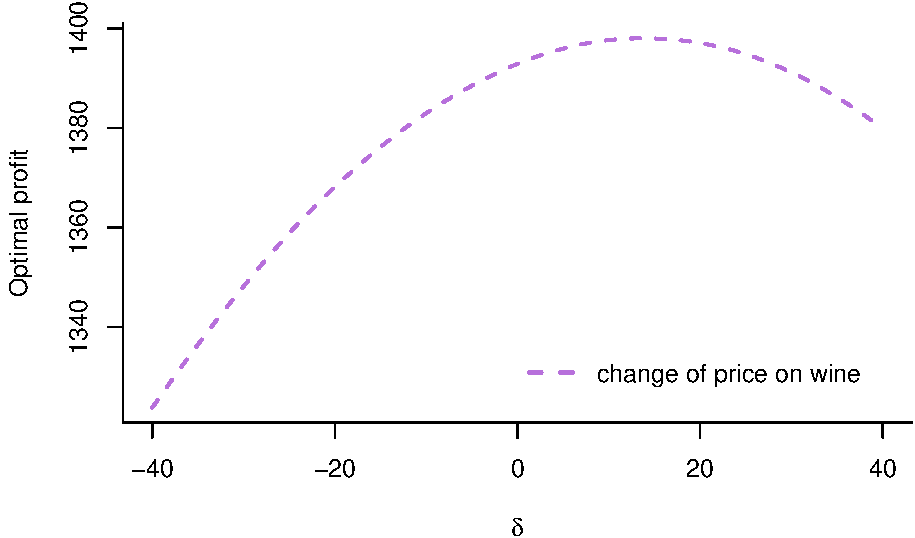
\includegraphics{real_case_files/figure-latex/price1_plot-1.pdf}

\begin{table}[H]
\centering
\resizebox{\linewidth}{!}{
\begin{tabular}{lccccccccccccccc}
\toprule
  & beer & wine & tea & bread & egg & fish & fruit & juice & vegetable & tobacco & meat & milk & coffee & dairy & oil\\
\midrule
maximum percentage of p decrease & 1 & 2 & 5 & 4 & 5 & 3 & 3 & 2 & 4 & 2 & 7 & 2 & 3 & 9 & 4\\
maximum percentage of p increase & 1 & 2 & 8 & 3 & 9 & 2 & 4 & 2 & 5 & 2 & 3 & 4 & 4 & 3 & 5\\
maximum percentage of std decrease & 7 & 14 & 100 & 100 & 100 & 100 & 7 & 100 & 6 & 100 & 100 & 100 & 100 & 100 & 100\\
\bottomrule
\end{tabular}}
\end{table}

\end{document}
